\chapter{Pulse Generator Measurements} \label{App:PulseGenTest}
This appendix presents a VHDL developed asynchronous pulse-generator, and the reasons not to use asynchronous designs.

This pulse generator is an old version of the pulse generator described in section \refq{subsec:Pulse_Generator} and the code for this one can be seen in appendix \refq{App:UnusedPulseGeneratorCode}.

The pulse generator module was tested on it's own to check if it will consistently generate pulses immediately following a trigger input. The whole code for this module can be found in appendix \refq{App:UnusedPulseGeneratorCode}. To do this an external 'trigger' input was added to the FPGA and and the 'active' and 'pulse' outputs were measured with an oscilloscope. The oscilloscope is a Rigol DHO924S and it was set to use one of it's 'deep memory' functions, called Ultra Acquire, in order to display several waveforms side by side. The pulse generator is set to produce exactly 6 pulses and the results of this can be seen on figure \refq{fig:A_PulseGen_Test}.

\begin{figure}[H]
    \centering
    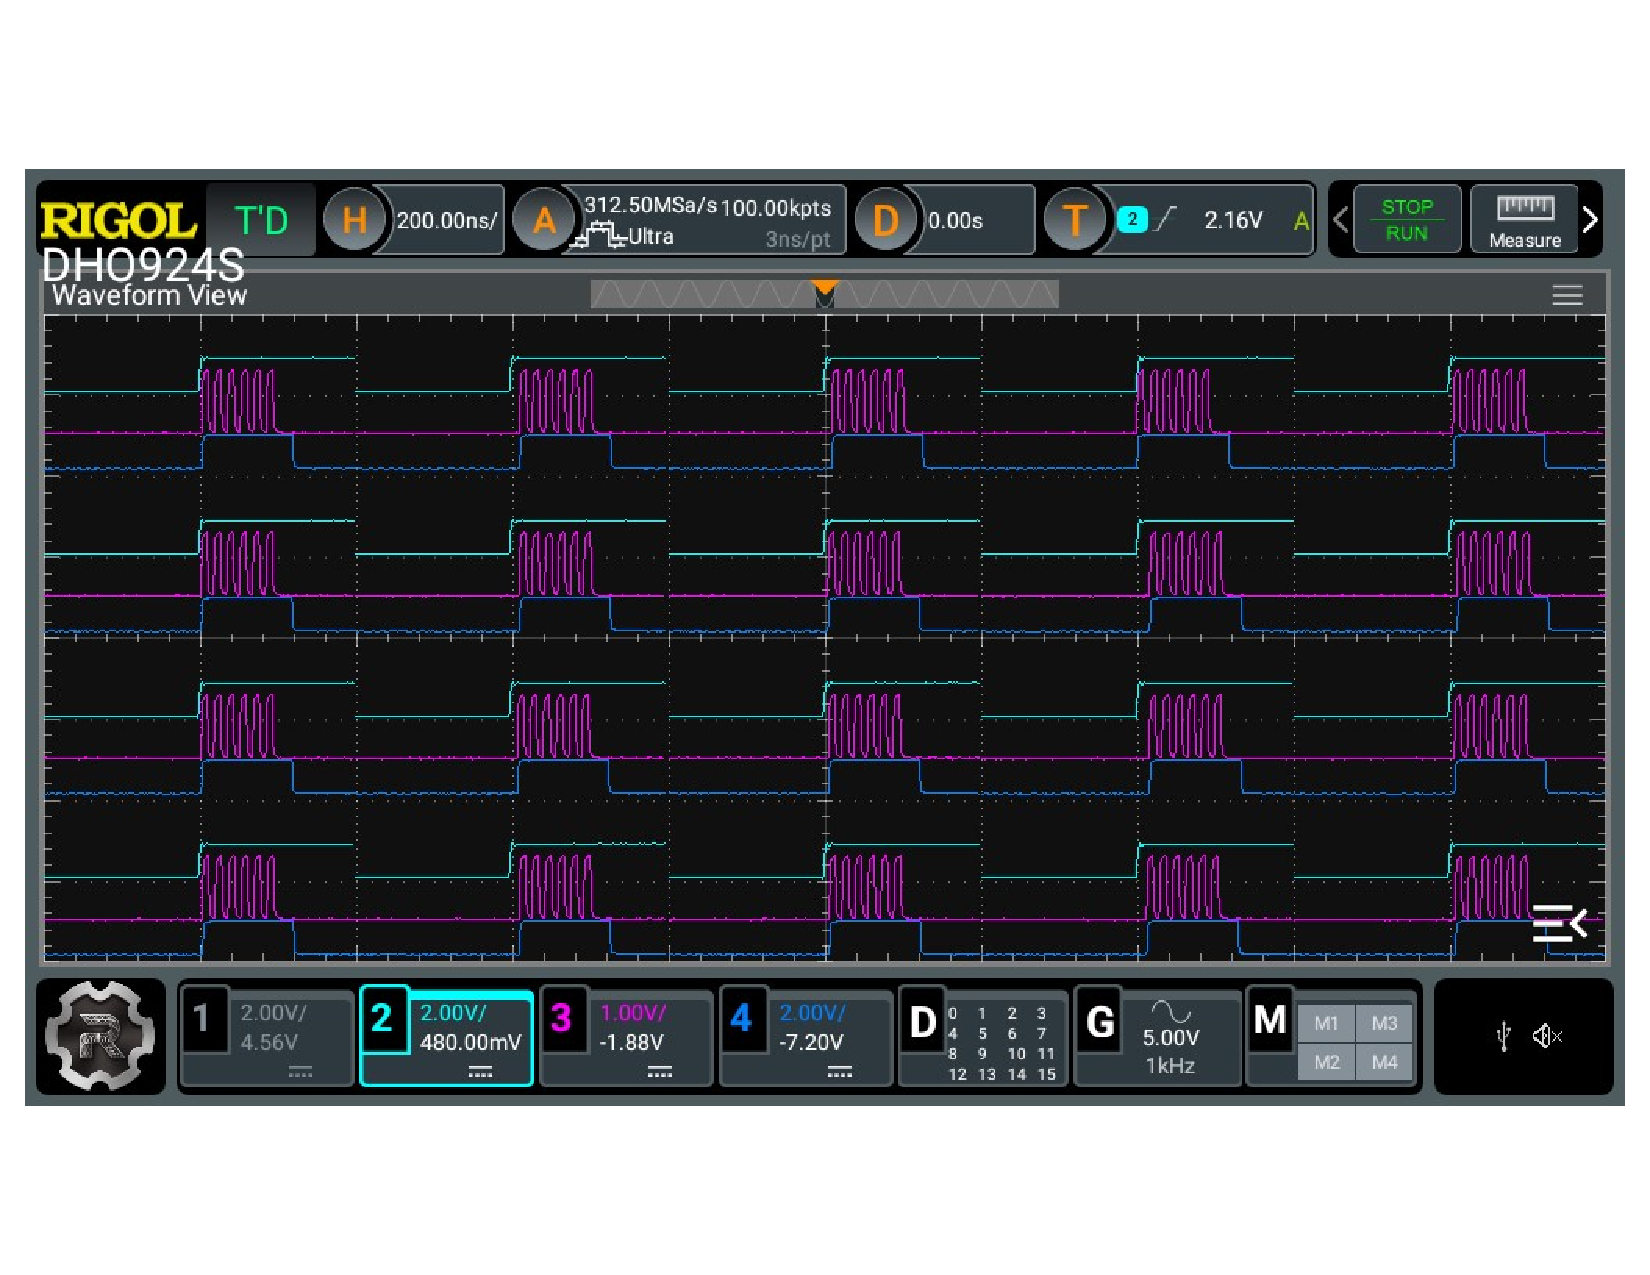
\includegraphics[clip, trim=0 50 0 50, width=1\textwidth]{Appendix/Figures/A_PulseGen_Test.pdf}
    \caption{An oscilloscope screenshot of the pulse generators 'trigger' input (cyan), active' output(blue) and 'pulse' output(red). The oscilloscope is using a deep memory 'ultra acquire' mode to display 20 consequtive readings in a 'mosaic' pattern.}
    \label{fig:A_PulseGen_Test}
\end{figure}

As can be seen on figure \refq{fig:A_PulseGen_Test} the pulse generator will always generate the desired amount of pulses, however it can be seen that the 'pulses' and 'active' signals are not asserted in a uniform way relative to the trigger input. They are often delayed from the trigger input by several nano seconds. This can occur because the assertion of the pulse generator from appendix \refq{App:UnusedPulseGeneratorCode} happens asynchronously to the main clock input. The pulse generator is thus not suitable for applications that have tight timing requirements. 